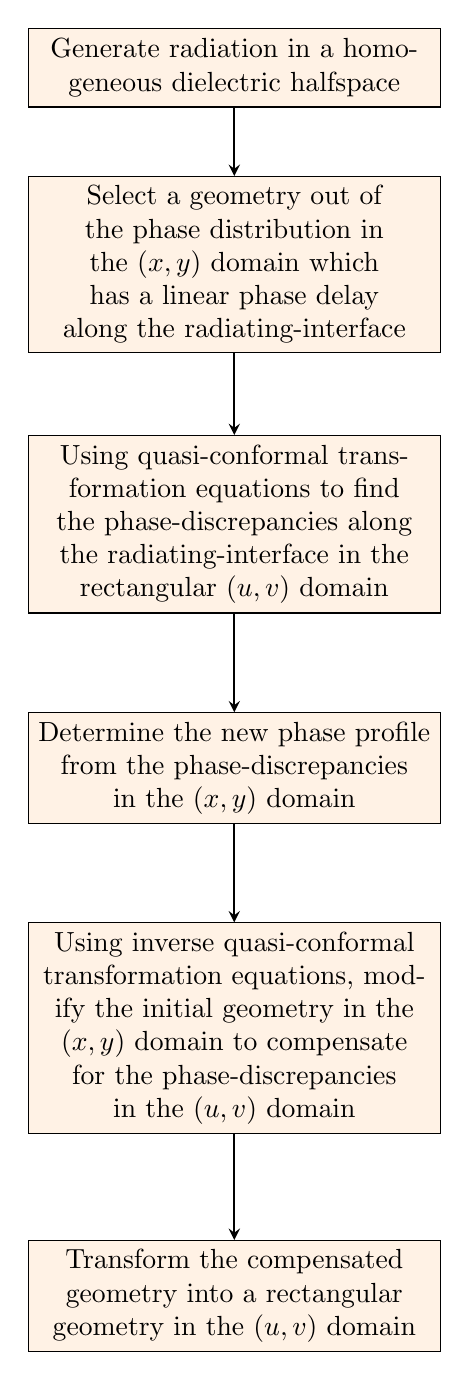
\begin{tikzpicture}[node distance=2cm]

\node (pro1) [rectangle, minimum width=3cm, minimum height=1cm, text centered, text width=5cm, draw=black, fill=orange!10] {Generate radiation in a homogeneous dielectric halfspace};
\node (pro2) [rectangle, minimum width=3cm, minimum height=1cm, text centered, text width=5cm, draw=black, fill=orange!10, below of=pro1, yshift=-.5cm] {Select a geometry out of the phase distribution in the $(x,y)$ domain which has a linear phase delay along the radiating-interface};
\node (pro3) [rectangle, minimum width=3cm, minimum height=1cm, text centered, text width=5cm, draw=black, fill=orange!10, below of=pro2, yshift=-1.3cm] {Using quasi-conformal transformation equations to find the phase-discrepancies along the radiating-interface in the rectangular $(u,v)$ domain};
\node (pro4) [rectangle, minimum width=3cm, minimum height=1cm, text centered, text width=5cm, draw=black, fill=orange!10, below of=pro3, yshift=-1.1cm] {Determine the new phase profile from the phase-discrepancies in the $(x,y)$ domain};
\node (pro5) [rectangle, minimum width=3cm, minimum height=1cm, text centered, text width=5cm, draw=black, fill=orange!10, below of=pro4, yshift=-1.3cm] {Using inverse quasi-conformal transformation equations, modify the initial geometry in the $(x,y)$ domain to compensate for the phase-discrepancies in the $(u,v)$ domain};
\node (pro6) [rectangle, minimum width=3cm, minimum height=1cm, text centered, text width=5cm, draw=black, fill=orange!10, below of=pro5, yshift=-1.4cm] {Transform the compensated geometry into a rectangular geometry in the $(u,v)$ domain};

\draw [thick,->,>=stealth] (pro1) -- (pro2);
\draw [thick,->,>=stealth] (pro2) -- (pro3);
\draw [thick,->,>=stealth] (pro3) -- (pro4);
\draw [thick,->,>=stealth] (pro4) -- (pro5);
\draw [thick,->,>=stealth] (pro5) -- (pro6);

\end{tikzpicture}
